% !TeX root = tcolorbox.tex
% include file of tcolorbox.tex (manual of the LaTeX package tcolorbox)
\clearpage
\section{Side by Side}\label{sec:sidebyside}%
\tcbset{external/prefix=external/sidebyside_}%

A \emph{side by side} box is a special \refEnv{tcolorbox} where
the upper and lower part of the box are set side by side.
All boxes of this kind are unbreakable.

\begin{marker}
  Further side by side options for code examples are
  \refKey{/tcb/listing side text},
  \refKey{/tcb/text side listing},
  \refKey{/tcb/listing outside text}, and
  \refKey{/tcb/text outside listing}.
\end{marker}

\subsection{Basic Settings}\label{subsec:sidebyside_basic}

\begin{docTcbKey}{sidebyside}{\colOpt{=true\textbar false}}{default |true|, initially |false|}
Normally, the upper part and the lower part of the box have their positions
as their names suggest. If |sidebyside| is set to |true|, the upper part
is drawn \emph{left-handed} and the lower part is drawn \emph{right-handed}.
Both parts are drawn together with the geometry settings of the upper part but the
space is divided horizontally according to the following options.
Colors, fonts, and box content additions are used individually.
The resulting box is unbreakable.

\begin{dispExample}
\tcbset{colback=red!5!white,colframe=red!75!black,fonttitle=\bfseries}

\begin{tcolorbox}[title=My title,sidebyside]
  This is the upper (\textit{left-handed}) part.
\tcblower
  This is the lower (\textit{right-handed}) part.
\end{tcolorbox}
\end{dispExample}


\begin{dispExample}
% \usepackage{lipsum}
% \tcbuselibrary{skins}
\begin{tcolorbox}[bicolor,sidebyside,righthand width=3cm,
    sharp corners,boxrule=.4pt,colback=green!5,colbacklower=green!50!black!50]
  \lipsum[2]
\tcblower
  
\includegraphics[width=\linewidth]{goldshade}%
\end{tcolorbox}
\end{dispExample}
\end{docTcbKey}



\clearpage
\begin{docTcbKey}[][doc updated=2015-02-06]{sidebyside align}{=\meta{alignment}}{no default, initially |center|}
  Sets the vertical \meta{alignment} for the left-handed and right-handed part.

  Feasible values for \meta{alignment} are:
  \begin{itemize}
  \item\docValue{center}: identical to |minipage| option |c|.
  \item\docValue{top}:    identical to |minipage| option |t| (aligns the top
      lines of the left-handed and right-handed side according to their baselines).
  \item\docValue{bottom}: identical to |minipage| option |b| (aligns the bottom
      lines of the left-handed and right-handed side according to their baselines).
  \item\docValue{center seam}: aligns the center of the left-handed and right-handed side.
  \item\docValue{top seam}:    aligns the very top seam of the left-handed and right-handed side.
  \item\docValue{bottom seam}: aligns the very bottom seam of the left-handed and right-handed side.
  \end{itemize}

\begin{exdispExample}{sidebyside_align}
\tcbset{colback=red!5!white,colframe=red!75!black,fonttitle=\bfseries,nobeforeafter,
  left=2mm,right=2mm,sidebyside,sidebyside gap=6mm,width=(\linewidth-2mm)/3}

\begin{tcolorbox}[adjusted title=center,sidebyside align=center]
This is a text which is too long for one line.
\tcblower
This is a short text.
\end{tcolorbox}\hfill
\begin{tcolorbox}[adjusted title=top,sidebyside align=top]
This is a text which is too long for one line.
\tcblower
This is a short text.
\end{tcolorbox}\hfill
\begin{tcolorbox}[adjusted title=bottom,sidebyside align=bottom]
This is a text which is too long for one line.
\tcblower
This is a short text.
\end{tcolorbox}
\end{exdispExample}


\docValue{center}, \docValue{top}, and \docValue{bottom} are identical
to the known corresponding |minipage| options.
While this is the preferred approach for text content, the result for
boxed content like tables or images may not be as expected.

For such content, one may use \docValue{center seam}, \docValue{top seam},
and \docValue{bottom seam}. For example, \docValue{top seam} aligns
the very top seam of the left-handed and right-handed side.


\begin{dispExample}
\tcbset{colback=red!5!white,colframe=red!75!black,fonttitle=\bfseries,
  size=small,righthand width=4cm,sidebyside,sidebyside gap=6mm,lower separated=false}

\begin{tcolorbox}[adjusted title=center seam,sidebyside align=center seam]
  This is my description text for the pictures displayed on the right-handed side.
  \tcblower
  
\includegraphics[width=\linewidth/2]{goldshade}%
  
\includegraphics[width=\linewidth/2]{blueshade}
\end{tcolorbox}

\begin{tcolorbox}[adjusted title=top seam,sidebyside align=top seam]
  This is my description text for the pictures displayed on the right-handed side.
  \tcblower
  
\includegraphics[width=\linewidth/2]{goldshade}%
  
\includegraphics[width=\linewidth/2]{blueshade}
\end{tcolorbox}

\begin{tcolorbox}[adjusted title=bottom seam,sidebyside align=bottom seam]
  This is my description text for the pictures displayed on the right-handed side.
  \tcblower
  
\includegraphics[width=\linewidth/2]{goldshade}%
  
\includegraphics[width=\linewidth/2]{blueshade}
\end{tcolorbox}
\end{dispExample}



\end{docTcbKey}

\clearpage
\begin{docTcbKey}{sidebyside gap}{=\meta{length}}{no default, initially |10mm|}
Sets the horizontal distance between the left-handed and right-handed part to
\meta{length}.
\begin{dispExample}
\tcbset{colback=red!5!white,colframe=red!75!black,fonttitle=\bfseries,nobeforeafter,
  sidebyside,width=(\linewidth-2mm)/2}

\begin{tcolorbox}[adjusted title=Wide gap,sidebyside gap=30mm]
This is a text which is too long for one line.
\tcblower
This is a short text.
\end{tcolorbox}\hfill
\begin{tcolorbox}[adjusted title=Narrow gap,sidebyside gap=1mm]
This is a text which is too long for one line.
\tcblower
This is a short text.
\end{tcolorbox}
\end{dispExample}
\end{docTcbKey}


\begin{docTcbKey}{lefthand width}{=\meta{length}}{no default, initially unset}
Sets the width of the left-handed part to the given \meta{length}.
\begin{dispExample}
\tcbset{colback=red!5!white,colframe=red!75!black,fonttitle=\bfseries}

\begin{tcolorbox}[title=My title,sidebyside,lefthand width=3cm]
This is the upper (\textit{left-handed}) part.
\tcblower
This is the lower (\textit{right-handed}) part.
\end{tcolorbox}
\end{dispExample}
\end{docTcbKey}

\enlargethispage*{1cm}
\begin{docTcbKey}{righthand width}{=\meta{length}}{no default, initially unset}
Sets the width of the right-handed part to the given \meta{length}.
\begin{dispExample}
\tcbset{colback=red!5!white,colframe=red!75!black,fonttitle=\bfseries}

\begin{tcolorbox}[title=My title,sidebyside,righthand width=3cm]
This is the upper (\textit{left-handed}) part.
\tcblower
This is the lower (\textit{right-handed}) part.
\end{tcolorbox}
\end{dispExample}
\end{docTcbKey}

\clearpage
\begin{docTcbKey}{lefthand ratio}{=\meta{fraction}}{no default, initially |0.5|}
Sets the width of the left-handed part to the given \meta{fraction} of
the available space. \meta{fraction} is a value between |0| and |1|.
\begin{dispExample}
\tcbset{colback=red!5!white,colframe=red!75!black,fonttitle=\bfseries}

\begin{tcolorbox}[title=My title,sidebyside,lefthand ratio=0.25]
This is the upper (\textit{left-handed}) part.
\tcblower
This is the lower (\textit{right-handed}) part.
\end{tcolorbox}
\end{dispExample}
\end{docTcbKey}


\begin{docTcbKey}{righthand ratio}{=\meta{fraction}}{no default, initially |0.5|}
Sets the width of the right-handed part to the given \meta{fraction} of
the available space. \meta{fraction} is a value between |0| and |1|.
\begin{dispExample}
\tcbset{colback=red!5!white,colframe=red!75!black,fonttitle=\bfseries}

\begin{tcolorbox}[title=My title,sidebyside,righthand ratio=0.25]
This is the upper (\textit{left-handed}) part.
\tcblower
This is the lower (\textit{right-handed}) part.
\end{tcolorbox}
\end{dispExample}
\end{docTcbKey}


\clearpage
If one side of a side-by-side box should be adapted to the width of
its content, this width has to be computed beforehand.
The following example uses a savebox |\mysavebox| to store the picture to determine
its width. A more convenient way to handle this task is to use the
methods from \Fullref{subsec:sidebyside_xparse}.

\begin{dispExample}
% \tcbuselibrary{skins,xparse}
% \usepackage{lipsum}
% \newsavebox\mysavebox  % preamble
\DeclareTotalTColorBox{\mysidebox}{ O{} +m +m }{
  bicolor,colback=white,colbacklower=yellow!10,
  fonttitle=\bfseries,center title,
  sidebyside,
  code={\sbox{\mysavebox}{#2}},
  lefthand width=\wd\mysavebox,
  drop lifted shadow,
  #1
}
{\usebox{\mysavebox}\tcblower#3}

\mysidebox[title=The Triangle]{%
  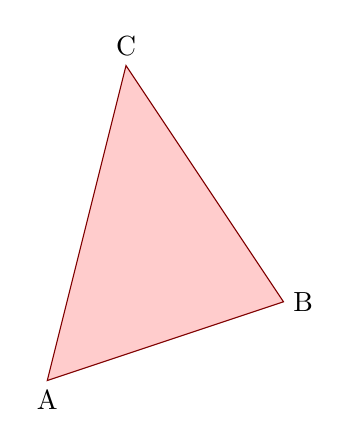
\begin{tikzpicture}
    \path[fill=red!20,draw=red!50!black]
      (0,0) node[below]{A} -- (3,1) node[right]{B}
      -- (1,4) node[above]{C} -- cycle;
  \end{tikzpicture}%
}{%
  \lipsum[1]
}
\end{dispExample}


\clearpage
\subsection{Advanced Settings from the \mylib{xparse} Library}\label{subsec:sidebyside_xparse}

\begin{marker}
All following macros and options need the \mylib{xparse} library to be
loaded, see \Fullref{sec:xparse}.
\end{marker}


\begin{docCommand}[doc new=2015-11-20]{tcbsidebyside}{\oarg{options}\marg{left-handed content}\marg{right-handed content}}
Creates a colored box using more or less arbitrary \meta{options} for a \refEnv{tcolorbox}.
The \refKey{/tcb/sidebyside} option is set to |true| and the
\meta{left-handed content} and \meta{right-handed content}
is filled into the box appropriately.
The resulting box is unbreakable.

\refCom{tcbsidebyside} is not only a shortcut for using
a normal \refEnv{tcolorbox} with \refKey{/tcb/sidebyside}, but allows
setting further options like \refKey{/tcb/sidebyside adapt}
and \refKey{/tcb/sidebyside switch}.


\begin{dispExample}
% \tcbuselibrary{skins,xparse}
% \usepackage{lipsum}
\tcbsidebyside[title=The Triangle,
  sidebyside adapt=left,
  bicolor,colback=white,colbacklower=yellow!10,
  fonttitle=\bfseries,center title,drop lifted shadow,
]{%
  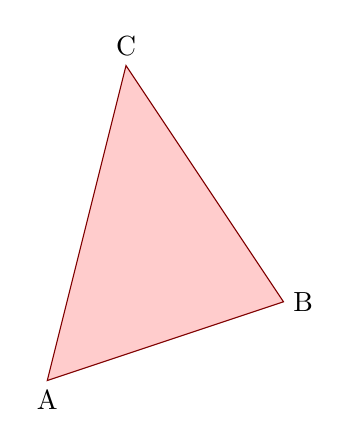
\begin{tikzpicture}
    \path[fill=red!20,draw=red!50!black]
      (0,0) node[below]{A} -- (3,1) node[right]{B}
      -- (1,4) node[above]{C} -- cycle;
  \end{tikzpicture}%
}{%
  \lipsum[1]
}
\end{dispExample}
\end{docCommand}


\clearpage
\begin{docTcbKey}[][doc new=2015-11-20]{sidebyside adapt}{=\meta{side(s)}}{no default, initially |none|}
The option allows the left-handed and/or right-handed side to determine the
dimensions of the box. This option is only valid inside \refCom{tcbsidebyside}.

Feasible values for \meta{side(s)} are:
\begin{itemize}
\item\docValue{none}: no measurement of left-handed and right-handed side.
\item\docValue{left}:
  the actual width of the left-handed content is used to set \refKey{/tcb/lefthand width}.
\item\docValue{right}:
  the actual width of the right-handed content is used to set \refKey{/tcb/righthand width}.
\item\docValue{both}:
  the actual width of the left-handed and right-handed content is used to set
  \refKey{/tcb/lefthand width}, \refKey{/tcb/righthand width}, and
  the overall \refKey{/tcb/width}.
\end{itemize}

\begin{dispExample}
% \tcbuselibrary{skins,xparse}
\tcbsidebyside[sidebyside adapt=left,
  title=Very important table,
  beamer,colframe=blue!50!black,colback=blue!10,
  lower separated=false,sidebyside gap=5mm
]{%
  \begin{tabular}{|l|c|r|}\hline
    left & center & right\\\hline
    A & B & C\\\hline
    D & E & F\\\hline
  \end{tabular}
}{%
  This table contains the most important figures for
  all future actions. You may notice that B follows A,
  C follows B, and so on.
}
\end{dispExample}



\begin{dispExample}
% \tcbuselibrary{skins,xparse}
\tcbsidebyside[sidebyside adapt=right,
  blanker,sidebyside gap=5mm
]{%
  \lipsum[2]
}{%

\begin{tikzpicture}
  \path[fill=yellow,draw=yellow!75!red] (0,0) circle (1cm);
  \fill[red] (45:5mm) circle (1mm);
  \fill[red] (135:5mm) circle (1mm);
  \draw[line width=1mm,red] (215:5mm) arc (215:325:5mm);
\end{tikzpicture}
}
\end{dispExample}


\begin{dispExample}
% \tcbuselibrary{skins,xparse}
\tcbsidebyside[sidebyside adapt=both,
  enhanced,center,
  title=Both sides adapted,
  attach boxed title to top center={yshift=-2mm},
  coltitle=black,boxed title style={colback=red!25},
  segmentation style=solid,colback=red!5,colframe=red!50
]{%
  \begin{tabular}{|l|c|r|}\hline
    left & center & right\\\hline
    A & B & C\\\hline
    D & E & F\\\hline
  \end{tabular}
}{%

\begin{tikzpicture}
  \path[fill=yellow,draw=yellow!75!red] (0,0) circle (1cm);
  \fill[red] (45:5mm) circle (1mm);
  \fill[red] (135:5mm) circle (1mm);
  \draw[line width=1mm,red] (215:5mm) arc (215:325:5mm);
\end{tikzpicture}
}
\end{dispExample}

\end{docTcbKey}


\clearpage
\begin{docTcbKey}[][doc new=2015-11-20]{sidebyside switch}{\colOpt{=true\textbar false}}{default |true|, initially |false|}
If set to |true|, the
\meta{left-handed content} and \meta{right-handed content}
of \refCom{tcbsidebyside} are switched.
Obviously, this option is only valid inside \refCom{tcbsidebyside}.

The side switching can be made even/odd page sensitive, if used inside
\refKey{/tcb/if odd page}.

\begin{dispExample}
% \tcbuselibrary{skins,xparse}
\tcbsidebyside{Left}{Right}

\tcbsidebyside[sidebyside switch]{Left}{Right}

\tcbsidebyside[title=Very important table,
  if odd page={sidebyside switch,sidebyside adapt=right,flushright title}%
              {sidebyside adapt=left},
  beamer,colframe=blue!50!black,colback=blue!10,
  lower separated=false,sidebyside gap=5mm
]{%
  \begin{tabular}{|l|c|r|}\hline
    left & center & right\\\hline
    A & B & C\\\hline
    D & E & F\\\hline
  \end{tabular}
}{%
  This table contains the most important figures for
  all future actions. You may notice that B follows A,
  C follows B, and so on.
}
\end{dispExample}


\end{docTcbKey}

